\documentclass[12pt]{article}
\usepackage[utf8]{inputenc}
\usepackage[frenchb]{babel}
\usepackage{listings}
\lstset{language=Java}
\RequirePackage[usenames,dvipsnames,xcolor=pst]{pstricks}
\RequirePackage{epsfig} % for eps fig
\RequirePackage{pst-blur} % for nice shadow
\RequirePackage{pst-dbicons} % for E/R
%\RequirePackage{mon-pst-uml} % for my own UML package
\RequirePackage{pst-uml} % for my own UML package
\RequirePackage{tikz} % circles such as History pseudostate
\newcommand{\monpsgrid}{\psgrid}
%\newcommand{\monpsgrid}{}
\setlength{\topmargin}{-5mm}%
\setlength{\oddsidemargin}{-1mm}%
\setlength{\evensidemargin}{-1mm}%
\setlength{\textwidth}{15.5cm}%
\setlength{\textheight}{8.9in}%
%------------------------------------      
%   QCM
%------------------------------------      
%\usepackage[french,correction]{qcm} % to print correct answers
%\usepackage[french]{qcm}
\title{\vspace{-3pc}\textbf{Contr\^ole M2104--BCOO}}

\date{Mercredi 15 juin 2016 -- Une seule feuille A4 manuscrite autoris\'ee\\
Dur\'ee : 1h30}

\def\dc{\textsf{Diagramme de Classe}}
\def\uc{\textsf{Diagramme de Cas d'Utilisation}}
\def\sni{\textsf{SNI}}
\def\ds{\textsf{Diagramme de S\'equence}}
\def\dss{\textsf{diagramme de S\'equence Syst\`eme}}
%===========================================================
\begin{document}
\maketitle

\section*{Description}

Votre rôle est de spécifier un nouveau système informatique à embarquer dans toutes les  voitures connectées : MyWaze\footnote{Merci à Mireille Blay-Fornarino, du département informatique de l'IUT de l'Université de Nice Sophia Antipolis pour ce sujet.}!

Vous avez vu un GPS? Vous avez utilisé GoogleMap? Vous connaissez Waze? Au volant, pas  toujours facile à utiliser\ldots{} 
Vous avez déjà Twitté? Vous avez parfois envoyé un email, un SMS?  Envoyé une photo sur Instagram? 
Jamais en conduisant évidemment !! 
Et bien nous allons  construire un boitier embarqué dans votre voiture qui vous permettra de faire tout cela en  conduisant\footcite{Bien sûr tout au long du projet, nous vérifierons que ce boitier n’est pas une cause de danger, mais cela  n’est pas à prendre en compte dans le cadre de ce contrôle.}.

MyWase doit permettre à un ``conducteur'' de s’identifier, visualiser la carte, spécifier un itinéraire, d’envoyer un message, de recevoir un message.   
Un conducteur n’a pas  besoin de s’identifier pour demander à visualiser une carte, mais dans tous les autres cas  c’est  indispensable.  
Il  peut  s’identifier  soit  par  un  mot  de  passe,  soit  en  utilisant  des  périphériques extérieurs comme un lecteur d’empreintes digitales.  
Le conducteur doit  pouvoir commander le boitier à la voix ou au toucher. 
Un ``gentilAdministrateur'' peut configurer le boitier pour l’associer à un conducteur en  précisant les informations sur ses réseaux sociaux (par exemple, le compte ``chut'' sur Twitter, ``NSA" sur google+, etc.). 
Il doit également pouvoir créer de nouveaux modèles  de messages, dits ``créatifs", en modifier ou en détruire. 
Un modèle de messages peut  être soit prédéfini et dans ce cas, il s’agit des modèles de messages fournis par Waze  (accident,  bouchon, \ldots)  ,  soit  ``créatif"  et  dans ce  cas  nous nous  nous  limitons  aux  modèle de messages sur Twitter ou par Email.   
Dans tous les cas de modèles créatifs de  messages,  un  intitulé   est  associé  (par  exemple,  Retard),  un  identifiant  pour  la  reconnaissance vocale (par exemple, Late), une icône graphique (par  exemple, un  fichier \texttt{.png} correspondant à une montre cassée), un contenu (par exemple, ``je suis en retard") et l’ensemble des informations qui devront être associées au message  parmi  un  ensemble  prédéfini  : itinéraire, position courante, destination, heure d’arrivée prévue,  \ldots{}.
Par  exemple,  à  un  message  correspondant à un Retard, la position courante et l’heure d’arrivée prévue devront être  associées. 
La durée de tentative pour envoyer le message est aussi associée au modèle  de messages (par exemple pour un Retard,  5mn, car après c’est inutile). 
Dans le cas d’un  modèle de messages correspondant à des emails, l’adresse à laquelle envoyer les emails  (par exemple ``monPote@iut.fr")  est également définie. 
Dans le cas d’un modèle de  messages correspondant à des tweet, le compte Twitter à partir duquel les messages  doivent partir doit être précisé (par exemple, @surLaRoute).   
Si le compte n’a pas  encore été paramètré dans MyWaze, il peut l’être en cours de création du modèle de  messages. Sur la route, lorsque le conducteur sélectionne le modèle de messages ainsi créé (par  exemple  Retard),  le  système  envoie  automatiquement  le  message  contenant  les  informations associées (par exemple, dans le cas d’un Retard, un email :  A : monPote@iut.fr ; sujet : retard ;   contenu : ``je suis en retard. Je suis à (Latitude :  43.58, Longitude : 7.11). Je dois arriver vers 19h20., date envoi : 19h05").   
Cinq minutes plus tard le conducteur peut renvoyer un message et s’il a pu rouler, le  contenu du message sera alors ``je suis en retard. Je suis à (Latitude : 43.65, Longitude :  7.11). Je dois arriver vers 19h27., date envoi : 19h10". 
Si le système ne parvient pas à  envoyer le message, le message passe alors dans un état EnAttente. Le système re-tente  l’envoi pendant la durée prévue par le modèle du messages, en l'occurrence dans le cas  d’un  retard,  5mn.  
Lorsque  l’envoi  est  réussi,  le  message  est  détruit.  
Lorsque  l’envoi  échoue, le message passe dans l’état Echec.  
Nous envisageons que les modèles de messages fassent l’objet de jeux dans différentes  communautés : #voitureJauneCroisée, #NiceMonacoRecordDeLenteur, etc.
Pour envoyer un message, le conducteur déjà identifié dispose d’une interface dédiée  qui lui présente les différents modèles de messages possibles. 
Scénario : Le conducteur sélectionne le modèle de messages parmi les modèles connus  de son boitier\footnote{Il peut s’agir de toucher l’écran ou d’énoncer le modèle de messages ``Police" ou ``Late" par exemple. On considère que la même ``interface" (au sens Java) gère les deux types de communication.}. 
Le système construit le message, puis le lit. Le conducteur doit alors  valider l’envoi. 
Le message est alors envoyé par le système. 
Si le système ne parvient pas  à l’envoyer, il annonce le problème, puis re-essaie jusqu’à réussir ou que le délai associé  à  ce  modèle  de  message  soit  dépassé.  
Dans  ce  cas,  il  avertit  le  conducteur  que  le  message  n’est  pas  parti  par  un  signal  sonore.  
Inversement  dès  que  le  message  est  envoyé, le conducteur est averti.

\section*{Questions}

Les questions suivantes n'ont pas à être traitées dans l'ordre. Dessins au crayon à papier autorisé.

\subsection{Diagramme des Cas d'Utilisation}

Représentez acteurs et cas d’utilisation sur un diagramme. 

\subsection{Diagramme de Séquence}

Représenter  le  diagramme  de  séquence  correspondant  au  scénario.

\subsection{Diagramme de Classes}\label{mondc}

Construire un diagramme de classes qui représente le système en intégrant les  informations présentes dans l’ensemble des besoins exprimés précédemment.

\subsection{Codage d'un diagramme de classe}

En considérant le diagramme de classes de la figure \ref{dc} :

\begin{enumerate}
\item Justifiez la cardinalité 1 à partir des éléments présents dans le diagramme lui-même.
\item Donner la définition de la structure des classes  correspondantes en java.
\end{enumerate}

\begin{figure}
\scalebox{0.6}{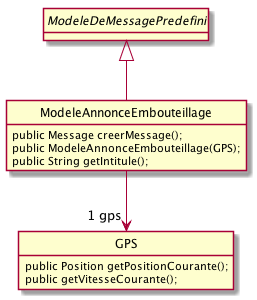
\includegraphics{exam2016}}
\caption{Un diagramme de classe}\label{dc}
\end{figure}

\subsection{Rétro-ingénierie d'un code Java}

Compléter  votre  diagramme  de  classe (section~\ref{mondc}) pour  prendre  en  compte  le  code  suivant\footnote{N’inventez pas. Si vous n’avez pas d’information, modélisez uniquement les informations dont vous disposez.}.

\begin{lstlisting}
public class FabriqueDeMessages extends Fabrique {
       public HashMap<String,ModeleDeMessage> modeles =
                                  new hashMap<String,ModeleDeMessage>();
       public Message creerMessage(String unModeleIntitule) {
             ModeleDeMessage mdm =  modeles.get(unModeleIntitule);
             if (mdm == null)
                    return null;
             else
                    return mdm.creerMessage();
}
       public boolean envoyer(Message unMessage) {
             return unMessage.envoyer();
}
       public boolean ajouterModeleDeMessage(ModeleDeMessage unModele){
             if (modeles.containsKey(unModele.getIntitule()) )
                           return false;
             else {
                    modeles.put(unModele.getIntitule(), unModele);
                    return true;
} }
}
\end{lstlisting}

%\newpage
\section*{Bar\`eme prévisionnel}

\begin{description}
\item[1] 4 points 
\item[2.1] 2 points 
\item[2.2] 4 points 
\item[2.2] 2 points 
\item[3] 10 points 
\end{description}

\end{document}
%===========================================================